\comment{Suggestion: past tense}\\

\subsection{Gradient Descent analysis}
    \begin{figure*}
        \begin{subfigure}{.5\textwidth}
            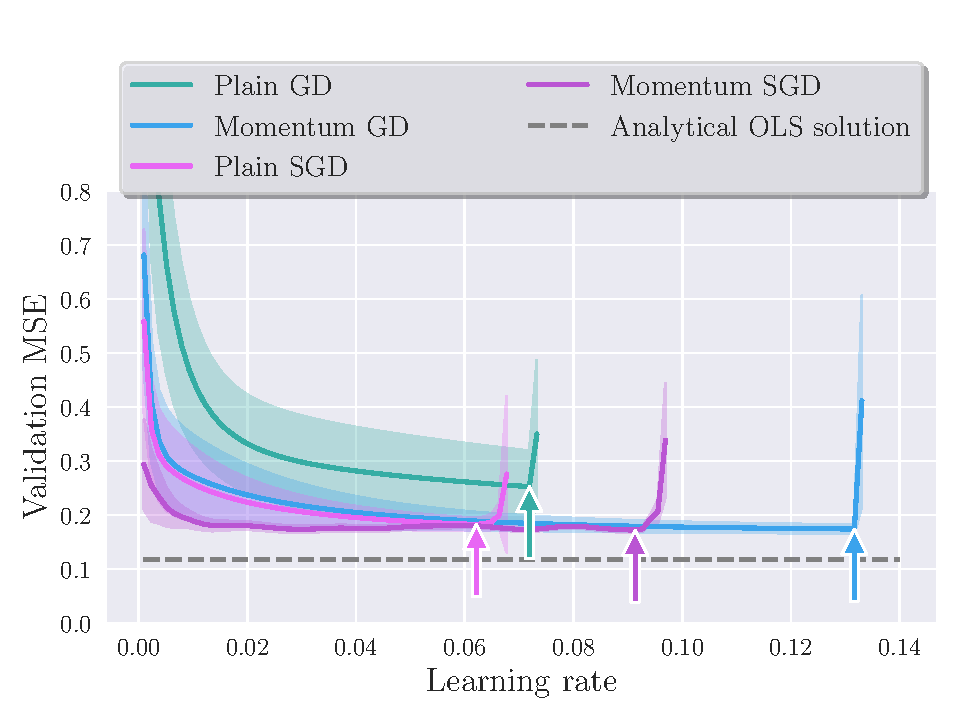
\includegraphics[width=\linewidth]{learning_rates_PGD_MGD_PSGD_MSGD.pdf}
            \caption{Best MSEs, learning rates: (0.2548, 0.03941), (0.1747, 0.126), (0.1795, 0.0384), (0.1761, 0.00874)}
            \label[fig]{res:fig:lrate1}
        \end{subfigure}
        \hfill
        \begin{subfigure}{.5\textwidth}
            \centering
            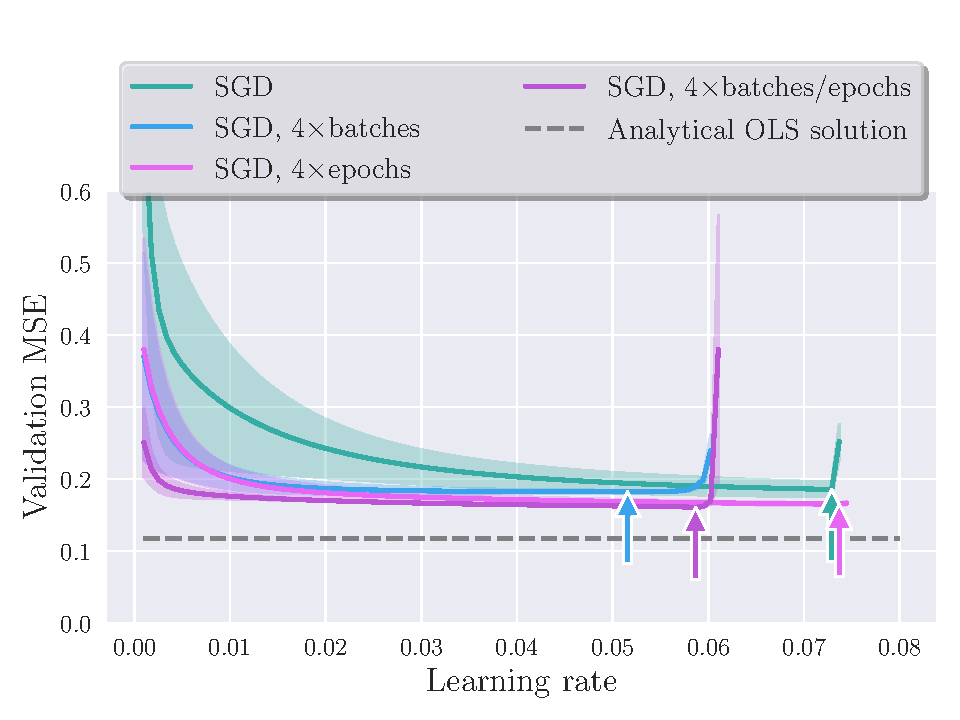
\includegraphics[width=\linewidth]{learning_rates_SGD_batches_epochs.pdf}
            \caption{Best MSEs, learning rates: (0.1795, 0.0382), (0.1750, 0.0152), (0.1712, 0.0329), (0.1703, 0.00345)}
            \label[fig]{res:fig:lrate2}
        \end{subfigure}
        \hfill
        \begin{subfigure}{.5\textwidth}
            \centering
            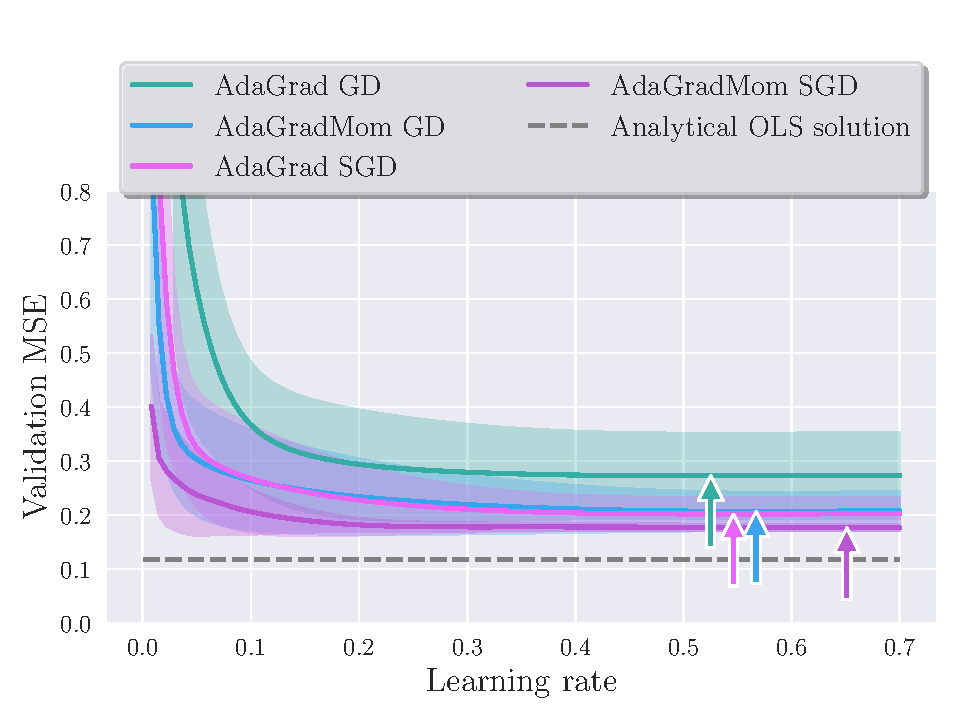
\includegraphics[width=\linewidth]{learning_rates_adagrad}
            \caption{Best MSEs, learning rates: (0.2748, 0.534), (0.2078, 0.570), (0.1827, 0.558), (0.1790, 0.180)}
            \label[fig]{res:fig:lrate3}
        \end{subfigure}
        \hfill
        \begin{subfigure}{.5\textwidth}
            \centering
            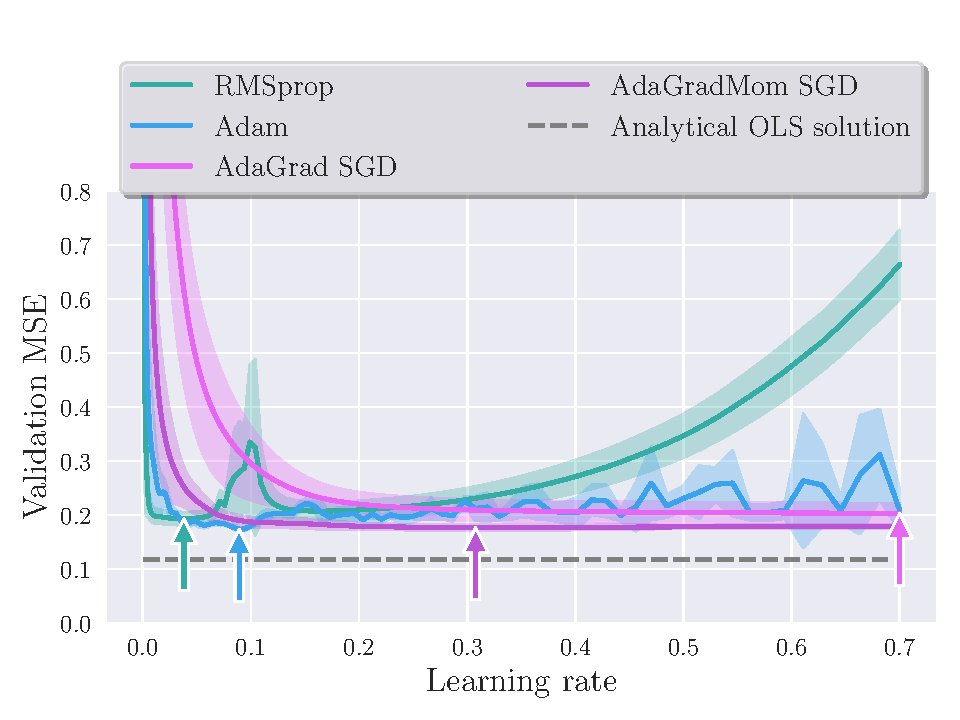
\includegraphics[width=\linewidth]{learning_rates_tunable}
            \caption{Best MSEs, learning rates: (0.1827, 0.558), (0.1790, 0.180), (0.1832, 0.00610), (0.1800, 0.0181)}
            \label[fig]{res:fig:lrate4}
        \end{subfigure}
        \caption{Plots of the validation MSE of the parameters found from optimising the OLS cost function on Franke function data with $n=600$ data points. For the momentum methods we used $\gamma=0.8$. The stochastic methods used 16 batches and 100 epochs, while the standard GD did 100 iterations unless specified otherwise.
        Analytical OLS MSE: 0.1178.}
        \label[fig]{res:fig:lrates}
    \end{figure*}